\section{Künstliche Intelligenz}
\label{chap:KI}

Das Thema \ac{KI} hat in letzter Zeit eine große mediale Aufmerksamkeit erhalten. Ein aktuelles Beispiel dafür ist der Chatbot ChatGPT der Firma OpenAI.
ChatGPT wurde im November 2022 veröffentlicht und ist ein Sprachmodell, das natürliche Sprache verstehen und abhängig von der 
Benutzereingabe in Dialogform Antworten liefern soll. Es ist dabei in der Lage, sich an vorherige Eingaben zu erinnern und kann 
deshalb Anfragen in einen Kontext einordnen. Dadurch kann es auch vorherige Antworten korrigieren und auf Wünsche und Bedürfnisse 
des Benutzers eingehen \cite[]{CHATGPT}. 

Die Frage nach \ac{KI} und nach dem ob und wie Maschinen denken können ist jedoch wesentlich älter als dieser Chatbot. 
Bereits Alan Turing stellte sich diese Frage in den 1950er Jahren. Er schlug vor, die Frage, ob Maschinen denken können,
mit einer anderen Frage zu ersetzen. Dafür formulierte er das Problem mithilfe eines Spiels, dem \glqq Imitation Game\grqq{}, 
das heute eher als Turing-Test bekannt ist, um. Dieses Spiel wird mit drei Personen gespielt, einem Fragesteller, einem Mann und 
einer Frau. Ziel des Spiels ist es, dass der Fragesteller mithilfe von Fragen herausfinden soll, welche Person der Mann und welche Person 
die Frau ist. Der Mann soll dabei versuchen, den Fragesteller dazu zu bringen, ihn fälschlicherweise als die Frau zu identifizieren, während die Frau versuchen soll, 
dass der Fragesteller sie korrekt als Frau identifiziert. Dafür befindet sich der Fragesteller in einem anderen Raum und die Fragen werden entweder 
über eine außenstehende weitere Person oder einem Fernschreiber übermittelt. Was würde nun passieren, wenn eine Maschine die Rolle des Mannes übernehmen würde?
Würde der Fragesteller dann häufiger oder seltener gewinnen? Alan Turing glaubte, dass eine Maschine dann als
intelligent bezeichnet werden könne, wenn eine Maschine in der Lage dazu wäre, menschliches Verhalten zu imitieren \cite[vgl. S.433f.]{TURING}.

\begin{figure}[H]
    \centering
    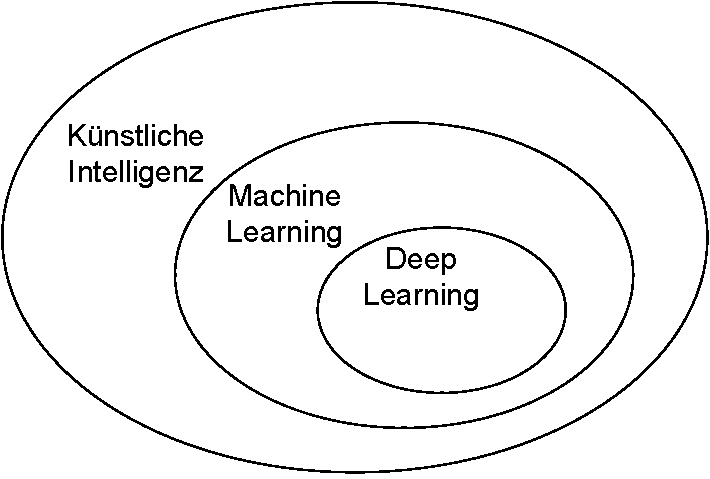
\includegraphics[width=\textwidth/2]{abbildungen/KI_ML_DL.pdf}
    \caption{Beziehung zwischen \acs{KI}, \acs{ML} und \acs{DL} \cite[S.22]{DL_PY}}
    \label{fig:KI_ML_DL}
\end{figure} 

François Chollet, der Entwickler der Deep-Learning-Bibliothek Keras, welche im Kapitel TODO näher beschrieben wird, definiert
das Fachgebiet \ac{KI} als \glqq [den] Versuch, normalerweise von Menschen erledigte geistige Aufgaben automatisiert zu lösen\grqq{} \cite[S.22]{DL_PY}.
Nach dieser Definition schließt \ac{KI} weitere Themen wie das \ac{ML} sowie das \ac{DL} ein. Wichtig zu beachten ist dabei,
dass diese Gebiete sich voneinander unterschieden. Ihre Beziehung zueinander wird in Abbildung \ref*{fig:KI_ML_DL} verdeutlicht.\\

Dieses Kapitel wird näher erläutern, worum es sich bei den Themen \ac{ML} und \ac{DL} handelt und wie ein \ac{KI}-Modell als neuronales Netz erstellt wird.

\subsection{Maschinelles Lernen}

Das maschinelle Lernen ist ein Teilgebiet der \ac{KI} und beschäftigt sich mit der Frage, ob ein Computer in der Lage dazu ist selbstständig eine bestimmte Aufgabe
zu erlernen. Ziel dabei ist es, dass eine Maschine aus einem vorgegebenem Datensatz und den dazugehörigen Antworten Regeln extrahieren soll, die den Datensatz erklären
können. Anders als bei der klassischen Programmierung soll eine Maschine hier nicht die Antworten aus den Daten und Regeln herausgeben, sondern selber nach einer
Struktur suchen, aus der die Maschine dann Regeln ableiten kann, die auch auf andere Aufgaben angewendet werden können \cite[vgl. S.23f.]{DL_PY}. Angenommen ein Datensatz bestünde aus
Bildern von Hunden und Menschen. Bei der klassischen Programmierung würde der Programmierer nun selber Regeln definieren und diese programmieren müssen. Beispiele für 
mögliche Regeln könnten hier sein:
\begin{quote}
    Wenn Wesen Fell hat, dann ist es ein Hund.\\
    Wenn Wesen auf zwei Beinen läuft, dann ist es ein Mensch.
\end{quote}
Beim \ac{ML} hingegen müsste der Programmierer diese Regeln nicht selber definieren. Hier werden neben dem Datensatz noch die entsprechenden Antworten benötigt. 
Jedes Bild bräuchte also ein Label, also eine Information darüber, ob es sich auf dem Bild um einen Hund oder einen Menschen handelt. Aufgabe der Maschine wäre es nun, 
mithilfe des Datensatzes und der Label, Regeln zu definieren, ob auf einem Bild ein Hund oder ein Mensch zu sehen ist. Das \ac{ML}-System wird also sozusagen trainiert. 
Dem trainiertem System können dann neue Bilder gezeigt werden und es wäre in der Lage anhand seiner definierten Regeln vorherzusagen, ob auf den neuen Bildern Hunde oder 
Menschen zu sehen sind. 

\begin{figure}[H]
    \centering
    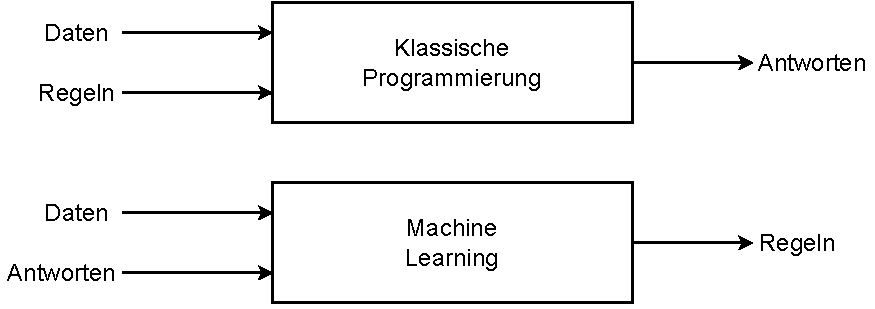
\includegraphics[scale=0.7]{abbildungen/Programmierparadigmen.pdf}
    \caption{Unterschiedliche Programmierparadigmen \cite[S.23]{DL_PY}}
    \label{fig:Programmierparadigma}
\end{figure}

Abbildung \ref*{fig:Programmierparadigma} verdeutlicht nochmal die Unterschiede zwischen der klassischen Programmierung und dem \ac{ML}. Beim \ac{ML} sind also drei Elemente
notwendig, diese werden anhand des oben genannten Beispiels verdeutlicht: 

\begin{description}[style=multiline,leftmargin=3cm,font=\bfseries]
    \item[Eingabedaten] Bilder von Menschen und Hunden \cite[S.24]{DL_PY}
    \item[Antworten] Label, ob auf dem Bild ein Mensch oder ein Hund abgebildet ist \cite[S.24]{DL_PY}
    \item[Metrik zur Bewertung des Algorithmus] Benötigt, um die Abweichung zwischen Ausgabe des Modells und eigentlicher Antwort zu bestimmen. Wird als Feedback-Signal genutzt,
    um Algorithmus anzupassen. Beispielsweise wie viel Prozent der Bilder richtig zugeordnet werden. \cite[S.24f.]{DL_PY}.  
\end{description}

Die Aufgabe eines \ac{ML}-Modells ist es passende Repräsentationen der Eingabedaten zu erlernen, das heißt, dass die Daten vom Modell sinnvoll umgewandelt werden müssen. 
Die systematische und automatische Suche nach der bestmöglichen Repräsentationen der Daten, mithilfe eines Feedback-Signals, für eine bestimmte vorgegebene Aufgabe kann als Möglichkeit 
verstanden werden, wie Maschinen lernen können. Mithilfe dieses Ansatzes und der in den letzten Jahren besser werdenden Hardware können große Datenmengen analysiert werden, was das Lösen von 
Aufgaben wie der Spracherkennung oder dem autonomen Fahren ermöglicht hat \cite[vgl. S.24ff.]{DL_PY}.\\

Die hier beschriebene Variante des Machine Learnings wird auch Supervised Learning, also überwachtes Lernen, genannt. \glqq Supervised\grqq{} bezieht sich hierbei darauf, dass
dem Modell die Antworten vorgegeben werden und es anhand der Antworten versucht Regeln zu finden. Neben dieser Variante existiert auch noch das sogenannte
Unsupervised Learning. Bei dieser Variante des Machine Learnings werden dem Modell keine Antworten gegeben. Stattdessen versucht das Modell die Daten anhand ihrer
Beziehung zueinander zu analysieren und die Daten in Kategorien zu klassifizieren. Algorithmen zum Clustern von Datensätze sind typische Beispiele für das Unsupervised Learning
\cite[vgl. S.47ff.]{AI_Huawei}. In dieser Arbeit finden Unsupervised Learning Algorithmen oder Modelle keine Anwendung, deshalb ist mit \ac{ML} hier immer Supervised Learning gemeint.

\subsection{Deep Learning und neuronale Netze}
\label{chap:DL}
Wie Abbildung \ref*{fig:KI_ML_DL} zeigt, ist das \ac{DL} ein Teilgebiet des \ac{ML} und beschäftigt sich somit ebenfalls mit der Suche nach den bestmöglichen Repräsentationen von
Daten. Das Besondere am \ac{DL} ist, dass das Lernen des Modells in mehreren aufeinanderfolgenden Schichten, auch Layer genannt, stattfindet. Dabei können
beliebig viele Schichten eingesetzt werden. Die Anzahl an Schichten wird auch Tiefe des Modells genannt, was auch das \glqq Deep\grqq{} in \ac{DL} beschreibt. Je tiefer dabei eine Schicht liegt,
desto sinnvoller sollen die Repräsentationen werden \cite[vgl. S.27]{DL_PY}. François Chollet definiert \ac{DL} als \glqq Lernen durch schichtweise Repräsentationen oder 
Lernen durch hierarchische Repräsentationen\grqq{} \cite[S.27]{DL_PY}. \ac{DL}-Modelle werden in der Regel als \ac{NN} dargestellt, das aus beliebig vielen Schichten besteht, wobei
jedes \ac{NN} mindestens eine Eingabe- und eine Ausgabeschicht  besitzt, dazwischen kann es beliebig viele versteckte Schichten, die hidden Layer, beinhalten. 
Die versteckten Schichten sind für die Verarbeitung der Daten zuständig. Eine Schicht besteht dabei aus einer vom Ersteller des \ac{NN} ausgewählten Anzahl an Neuronen, die miteinander 
verbunden sind \cite[vgl. S.26]{NN}. In der Abbildung \ref*{fig:NN_Modell} wird der grundlegende Aufbau eines einfachen neuronalen Netzes dargestellt. 

\begin{figure}[H]
    \centering
    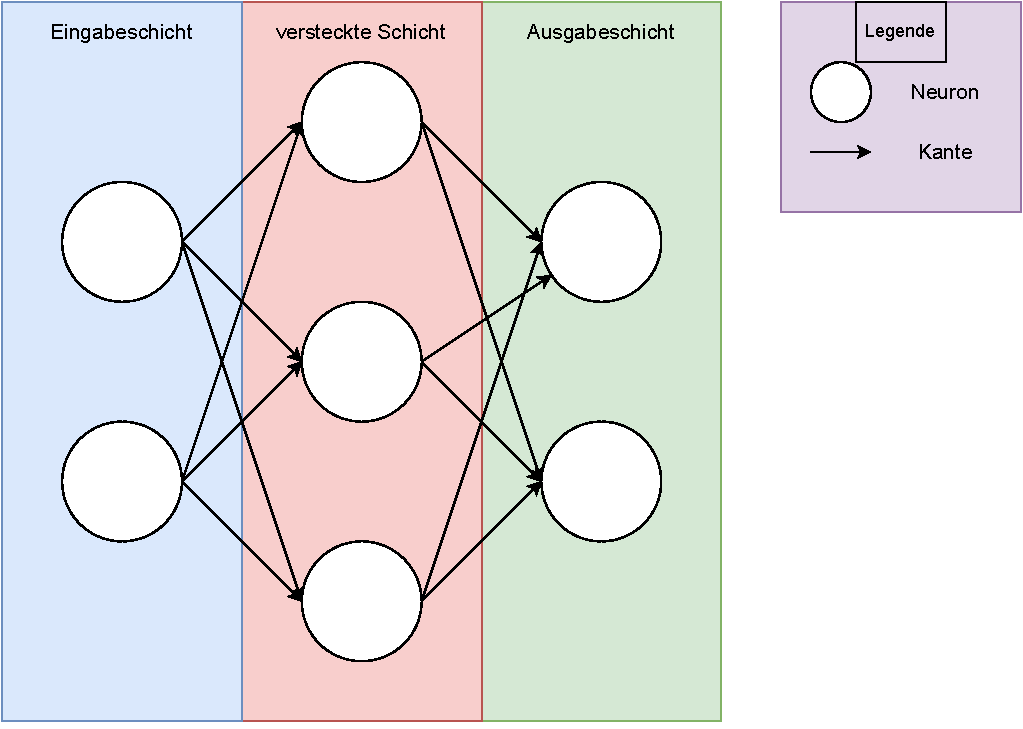
\includegraphics[scale=0.7]{abbildungen/NN_Modell.pdf}
    \caption{Aufbau eines neuronalen Netzes \cite[S.27]{NN}}
    \label{fig:NN_Modell}
\end{figure}

Die Verbindungen zwischen den Neuronen, die Kanten genannt werden, sind gerichtet und besitzen ein Gewicht. Wenn jedes Neuron eine Verbindung zu jedem Neuron in der nächsten Schicht hat, 
dann wird diese Schicht auch als fully-connected bezeichnet. Das \ac{NN} in Abbildung \ref*{fig:NN_Modell} besteht aus drei Schichten, welche, bis auf die Ausgabeschicht, 
fully-connected sind. Unabhängig davon bekommt jedes Neuron, welches sich nicht in der Eingabeschicht befindet, eine Netzeingabe, welche sich aus den Ausgaben der Neuronen zusammensetzt, 
die eine Kante zu dem jeweiligen Neuron haben. Dabei wird jede Ausgabe eines Neurons mit dem Kantengewicht multipliziert.

\begin{figure}[H]
    \centering
    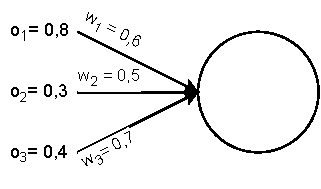
\includegraphics[width=\textwidth/2]{abbildungen/Aktivierungsfunktion.pdf}
    \caption{Berechnung Netzeingabe \cite[vgl. S.29]{NN}}
    \label{fig:Aktivierungsfunktion}
\end{figure}

Abbildung \ref*{fig:Aktivierungsfunktion} zeigt beispielhaft ein Neuron und die Ausgabe von drei vorherigen Neuronen. Die Netzeingabe des Neurons wird wie folgt berechnet \cite[S.29]{NN}:
\begin{align}
    net = o_{1} \cdot w_{1} + o_{2} \cdot w_{2} + o_{3} \cdot w_{3} = 0,8 \cdot 0,6 + 0,3 \cdot 0,5 + 0,4 \cdot 0,7 = 0,91
\end{align}

Jedes Neuron besitzt eine Aktivierungsfunktion, welche mithilfe der Netzeingabe prüft, ob das jeweilige Neuron eine Ausgabe hat und welchen Wert diese annimmt. Es existieren viele
verschiedene Aktivierungsfunktionen, in dieser Arbeit wird die \ac{ReLU}-Funktion genutzt. Diese ist definiert als \cite[S.31]{NN}:
\begin{align}
    f(net) = max(0; net)
\end{align}

Diese Funktion nimmt die Netzeingabe und wenn die Netzeingabe positiv ist, dann wird die Netzeingabe als Ausgabe ausgegeben, ansonsten gibt das Neuron 0 als Ausgabe aus.
Eine \ac{ReLU}-Funktion als Aktivierungsfunktion eines Neurons zu benutzen ist typisch im Bereich des \ac{DL} \cite[vgl. S.31]{NN}.

Wie kommen nun die Kantengewichte zustande? Den Kanten werden zunächst zufällige Werte als Gewicht zugeordnet. Danach wird jede Eingabe an das Modell übergeben, die
daraufhin die einzelnen Layer durchläuft. Die Vorhersage wird nun mit dem tatsächlichen Wert an eine Verlustfunktion übergeben, welche dann den Verlustscore berechnet.
Für eine Regression, also die Vorhersage eines numerischen Wertes, bietet sich beispielsweise die Berechnung des mittleren quadratischen Fehlers (mean squared error) an.
Dieser Verlustscore wird als Feedback-Signal genutzt und gibt an, wie gut das Modell die Aufgabe lösen kann. Das \ac{DL}-Modell versucht während des Trainings diesen 
Wert zu minimieren, indem der Verlustscore an einen Optimierer übergeben wird, der anhand des Verlustscores die Gewichtungen der Kanten im \ac{NN} aktualisiert.
Am Anfang des Trainingsprozesses wird der Verlustscore relativ hoch sein, da die Kantengewichte zufällig ausgewählt wurden. Mit jeder neuen Eingabe werden die Kantengewichte
jedoch aktualisiert, was zur Folge hat, dass das Modell immer genauer wird und der Verlustscore somit abnimmt \cite[vgl. S.30ff.]{DL_PY}.
Abbildung \ref*{fig:AnlernenNN} zeigt dabei grafisch den Aufbau des Trainingsprozesses eines \ac{NN}. Je mehr Daten vorhanden sind, desto genauer kann das 
Modell somit werden. Die ImageNet-Datenbank mit ihren 1,4 Millionen Bilddateien hatte beispielsweise einen großen Einfluss auf den Erfolg von \ac{DL} \cite[vgl. S.45]{DL_PY}.
Wichtig zu beachten ist, dass der Datensatz in einen Trainings- und einen Testdatensatz aufgeteilt werden muss. Ein Modell darf niemals mit den Daten trainiert werden,
die auch zum Testen genutzt werden. Wird ein Datensatz nicht aufgeteilt, wird das Modell logischerweise beim Testen sehr gute Ergebnisse erzielen, da es die 
Testdaten bereits kennt. Der Testdatensatz wird zudem genutzt, um die Genauigkeit des Modells bei unbekannten Daten zu bestimmen. Dieser Schritt ist wichtig, da 
so geprüft werden kann, wie gut ein Modell mit neuen Daten umgehen kann und ob es in der Lage ist diese korrekt vorherzusagen.

\begin{figure}[H]
    \centering
    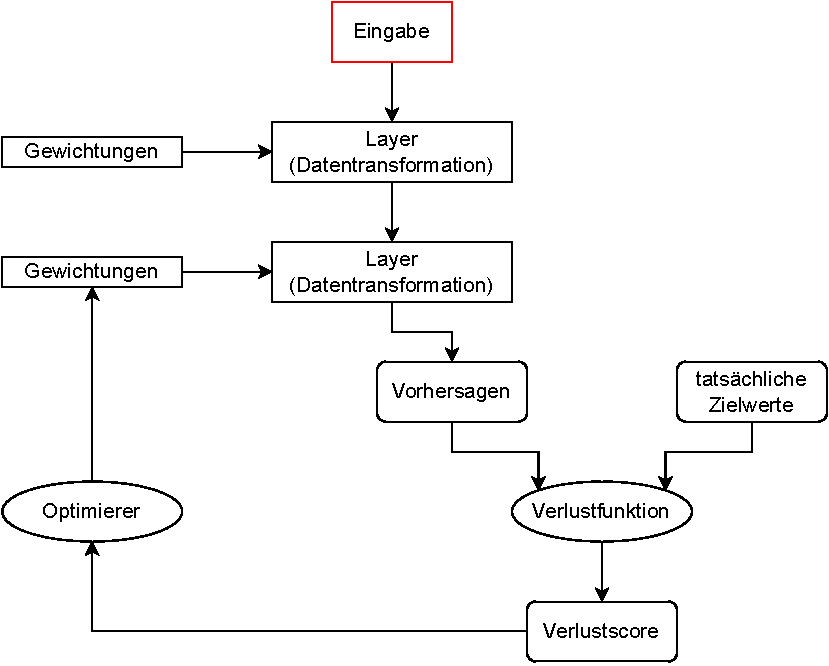
\includegraphics[width=\textwidth]{abbildungen/NN_anlernen.pdf}
    \caption{Anlernen eines neuronalen Netzes \cite[S.31]{DL_PY}}
    \label{fig:AnlernenNN}
\end{figure}

\subsection{Overfitting und Underfitting}
Overfitting und Underfitting, auf Deutsch Über- und Unteranpassung, können im Trainingsprozesses von \ac{ML}- sowie \ac{DL}-Aufgaben auftreten.
Unter dem Begriff Underfitting wird verstanden, dass ein Modell noch nicht alle Zusammenhänge im Trainingsdatensatz erkannt und modelliert hat und somit der Verlustscore noch hoch ist, 
da das Modell für den Trainingsdatensatz noch keine sinnvollen Repräsentationen gefunden hat. Dieses Problem kann gelöst werden, indem die Anzahl an Trainingsdurchläufen erhöht oder 
die Komplexität des Modells erweitert wird, also weitere Schichten oder mehr Neuronen in einer Schicht hinzugefügt werden. Overfitting beschreibt dabei den Fall,
dass ein Model die Eigenheiten der Trainingsdaten sozusagen auswendig lernt und mögliche irrelevante Muster im Trainingsdatensatz erlernt. Das Problem daran ist, dass das Modell 
dann nicht mehr in der Lage ist, das eigentliche Problem generalisiert zu betrachten und neue Daten korrekt vorherzusagen. Mögliche Lösungen wäre dabei mehr Daten zu beschaffen
oder die Komplexität des Modells zu verringern. Zudem existiert ein Verfahren, das ebenfalls dabei hilft, Overfitting zu verhindern. Dieses Verfahren nennt sich 
Dropout-Regularisierung. Bei der Dropout-Regularisierung werden während des Trainings einige zufällig ausgewählte Ausgaben von Neuronen in einer Schicht auf 0 gesetzt. Das soll verhindern,
dass ein \ac{NN} irrelevante Muster im Trainingsdatensatz erlernt \cite[vgl. S.142ff.]{DL_PY}. 

Je weniger Daten vorhanden sind und je komplexer ein Modell ist, desto wahrscheinlicher läuft das Modell Gefahr, von Overfitting betroffen zu sein. Je simpler ein Modell ist und je weniger
Trainingsdurchläufe durchlaufen werden, desto eher kann es zu einer Unteranpassung des Modells kommen. Es ist also wichtig, ein gutes Mittelmaß zu finden, damit ein Modell in der Lage ist
ein Problem verallgemeinert und optimal lösen zu können.

\subsection{Vor- und Nachteile}
Der große Vorteil von \ac{DL} und \ac{NN} ist das \glqq Universal Approximation Theorem\grqq{}, welches besagt, dass jeder funktionale Zusammenhang zwischen Ein- und Ausgabe
durch ein \ac{NN} angenähert werden kann. Das gilt dabei nicht nur für mathematische Zusammenhänge. Voraussetzung dafür ist ein \ac{NN}, dessen Komplexität groß genug gewählt wird. 
Dafür kann bereits eine versteckte Schicht ausreichen. Durch diese Eigenschaft kann ein \ac{NN} theoretisch jedes Approximationsproblem lösen und interessiert sich dabei nicht dafür, 
ob eine Kausalität zwischen Ein- und Ausgabe besteht und kann ebenfalls mit unvollständigen und falschen Daten arbeiten \cite[vgl. S.74ff.]{NN}. Zudem sind \ac{NN} nicht anfällig 
gegenüber leichten Änderungen im Datensatz, stattdessen sind sie fehlertolerant. Selbst wenn ein Teil des Netzes funktionsunfähig werden sollte, spielt das keine allzu große Rolle,
da die Muster und Strukturen, welches ein Modell gelernt hat, auf das gesamte Netz verteilt ist. Diese Tatsache hat zudem den Vorteil, dass wenn neue Daten dazu kommen, nicht 
das gesamte Netz neu trainiert werden muss, sondern das bestehende Netz upgedatet werden kann \cite[vgl. S.82]{NN}. Weitere Vorteile von \ac{NN} sind ihre Einfachheit und Skalierbarkeit.
Das Erstellen eines Modells ist einfach und auf eine beliebige Größe skalierbar, weshalb \ac{NN} auch mit großen Datenmengen und einer Vielzahl an Attributen angelernt werden 
können \cite[vgl. S.47]{DL_PY}.

Neben den Vorteilen bringt die Nutzung von \ac{NN} auch einige Nachteile mit sich. Zum einen ist die Genauigkeit der Prognose eines Modells stark abhängig von der Qualität der Trainingsdaten.
Werden Attribute im Trainingsdatensatz genutzt, die irrelevant bei der Beschreibung des Problems sind, wirkt sich das negativ auf die Genauigkeit des Modells aus, weshalb eine
vorhergehende Analyse der Attribute, die sogenannte \glqq Feature Selection\grqq{}, unausweichlich ist. Zudem kann das Training eines \ac{NN} mit steigender Komplexität
zeit- und rechenintensiv werden, da die Anzahl an zu berechnenden Parametern bei steigender Komplexität zunimmt. Ein komplexeres Modell hat außerdem zur Folge, dass es nicht mehr 
möglich ist transparent und nachvollziehbar zu Verstehen, wie ein \ac{NN} eine Ausgabe berechnet. Außerdem muss beim Testen und Validieren eines Modells überprüft werden, 
ob das Modell nicht eventuell over- oder underfitted und somit nicht in der Lage ist, das zu lösende Problem hinreichend verallgemeinert abzubilden und somit auf neuen Daten
zu fehlerhaftem Verhalten neigt \cite[vgl. S.84ff.]{NN}.





